%=============================================================================
% SVM Appendix
% Copyright (c) 2018. Lester James V. Miranda
%
% This file is part of thesis-manuscript.
%
% thesis-manuscript is free software: you can redistribute it and/or modify
% it under the terms of the GNU General Public License as published by
% the Free Software Foundation, either version 3 of the License, or
% (at your option) any later version.
%
% thesis-manuscript is distributed in the hope that it will be useful,
% but WITHOUT ANY WARRANTY; without even the implied warranty of
% MERCHANTABILITY or FITNESS FOR A PARTICULAR PURPOSE.  See the
% GNU General Public License for more details.
%
% You should have received a copy of the GNU General Public License
% along with thesis-manuscript.  If not, see <http://www.gnu.org/licenses/>.
%
% Created by: Lester James V. Miranda <ljvmiranda@gmail.com>
%=============================================================================

\chapter{Support-Vector Machines} 
\label{AppendixDistributed}

\par We have been mentioning Support-Vector Machines (SVM) as our pipeline's
classifier, yet have not provided any opportunity to discuss how it works. In
this chapter, we'll review the intuition behind SVMs, discuss how the
hyperparameters $C$ and $\gamma$ affect classification, then describe how we
implemented a distributed SVM for faster inference in multilabel data.

\section{Review and Intuition on SVMs}

\begin{wrapfigure}{r}{0.46\textwidth}
  \centering
    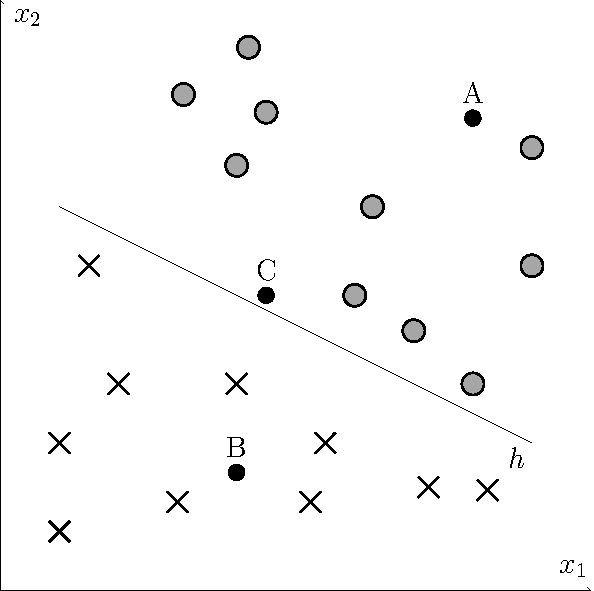
\includegraphics[width=0.45\textwidth]{appendix/svm_demo}
    \caption{Margin intuition for SVMs}
  \label{demo:svm}
\end{wrapfigure}

\par As an example, let's take a label $\lambda_1$ from our contrived protein
dataset (with only two features), and plot the samples on a Cartesian plane.
Figure \ref{demo:svm} shows the resulting plot.  The $\circ$ marks
represent protein samples that perform the function $\lambda_1$ (class 1),
whereas the $\times$ marks represent those that do not (class 0). We will also
draw a decision boundary $h$ that attempts to separate these classes.

\par If we query the unannotated sample $\mathbf{A}$, we can confidently infer
that it belongs to class 1. The same goes for sample $\mathbf{B}$, in this
case, class 0. However, we are on the fence with sample $\mathbf{C}$: it can
belong to class 1 according to the decision boundary, but it might as well be
class 0 if we nudge $h$ a bit. Our situation will be much better if we can
ensure that (1) our predictions are always \textbf{confident}, i.e. decision
boundary is maximally far from \textit{on-the-fence} samples, or
\textit{support vectors}, and that (2) they are \textbf{correct}, i.e., loss is
minimized. Ensuring that our decision-boundary makes confident and correct
predictions serves as the core machinery for the SVM classifier. We can write
this as an objective function $\gamma$:\footnote{\cite{ng2012support} gave a
thorough treatment of support-vector machines in his CS229 Lecture Notes. He
traces the development of SVMs from mere logistic regression up to Lagrangian
dualities and the kernel trick to solve the optimization problem.}

\begin{equation}
\begin{aligned}
\label{eqn:svm}
    & \underset{w,b}{\text{min}}
    & & \overbrace{\dfrac{1}{2}||w||^{2}}^{\mathclap{\text{confident}}} +
    C\overbrace{\sum_{i=1}^{m}{\xi_i}}^{\mathclap{\text{correct}}} \\
    & \text{s.t.}
    & & y^{(i)}(w^{T}x^{(i)} + b) \geq 1 - \xi_i, i=1,\dots,N \\
    &&& \xi_i \geq 0, i=1,\dots,N
\end{aligned}
\end{equation}

\par Without getting into the specifics of the objective function, we can see
that the hyperprameter $C$ is trying to balance our two goals: (1) ensuring
that the margin is far from the support-vectors by minimizing $||w||^{2}$, and
(2) checking that our predictions are correct. In addition, the parameters
$\{w, b\}$ are the same as the parameter $W$ learned during training in our
prediction pipeline (we simply let $b=w_0$). Lastly, we apply a kernel trick
to map our features with respect to the radial-basis function (RBF). Given two
samples $x$ and $z$, we write the RBF kernel as:

\begin{equation}
\label{eqn:kernel}
    K(x,z) = \text{exp} \left(-\gamma||x-z||^{2}\right)
\end{equation}

\par And thus we see the hyperparameter $\gamma$ that tries to consolidate the
\emph{effect} of each sample with respect to the other (measured in terms of
distance).\footnote{In some formulations, $\gamma=\dfrac{1}{\sigma^2}$} In the
next section, we will investigate the effect of the hyperparameters $C$ and
$\gamma$ in the behavior of our predictor.

\section{Practical Considerations for $C$ and $\gamma$ on the Decision Boundary}

\par From Equations \ref{eqn:svm} and \ref{eqn:kernel}, we can deduce the
effect of different hyperparameter settings to the decision boundary. The key
terms in this section are bias and variance, both refer to the generalizability
of the model.  Note that there is a tradeoff between bias and variance: too
high a bias underfits the model, while too high a variance overfits the model.

\begin{itemize}
    \item \textit{$C$ affects the way the margin is placed.} A \textbf{high}
        $\mathbf{C}$ will be motivated to predict more samples correctly than
        finding a large margin distance (high variance, low bias), but may fail
        to generalize well and perform poorly in the test set. On the other
        hand, a \textbf{low} $\mathbf{C}$ will strive to keep a good distance
        from support-vectors, but may suffer from severe underfitting (high
        bias, low variance).
    \item \textit{$\gamma$ affects the shape of the decision boundary.} The
        value of $\gamma$ controls each samples' area-of-effect. A
        decision-boundary with a \textbf{large} $\mathbf{\gamma}$ is only
        affected by the samples closest to it, creating a ``wiggly'' shape that
        conforms to the nearest samples (high variance, low bias). On the other
        hand, a \textbf{low} $\mathbf{\gamma}$ increases each samples'
        influence, thus even far-off samples are considered (high bias, low
        variance).
\end{itemize}

\par Figure \ref{demo:svm_hyperparams} demonstrates the effect of setting
different values for $C$ and $\gamma$ on a contrived binary dataset. We
randomly generated samples in two classes and ran SVM for different
hyperparameter settings then plotted the decision boundary for each
configuration. In the actual experiments, we first determined SVM hyperparameters
via grid search, then narrowed it down using fine random search.

\par We can see that a high-bias model ($C=1, \gamma=0.001$) underfits poorly
as it predicts everything as one class. On the other hand, a high-variance
model ($C=100, \gamma=1.0$) resembles the exact dumbell shape of the dataset.
Interestingly, the best performance for this simulation (3-fold
cross-validation) is from the high-variance model. This demonstration also
confirms our deductions: high $C$ or $\gamma$ values lead to high-variance models,
while low values lead to high-bias ones.


\begin{figure}[t]
  \centering
    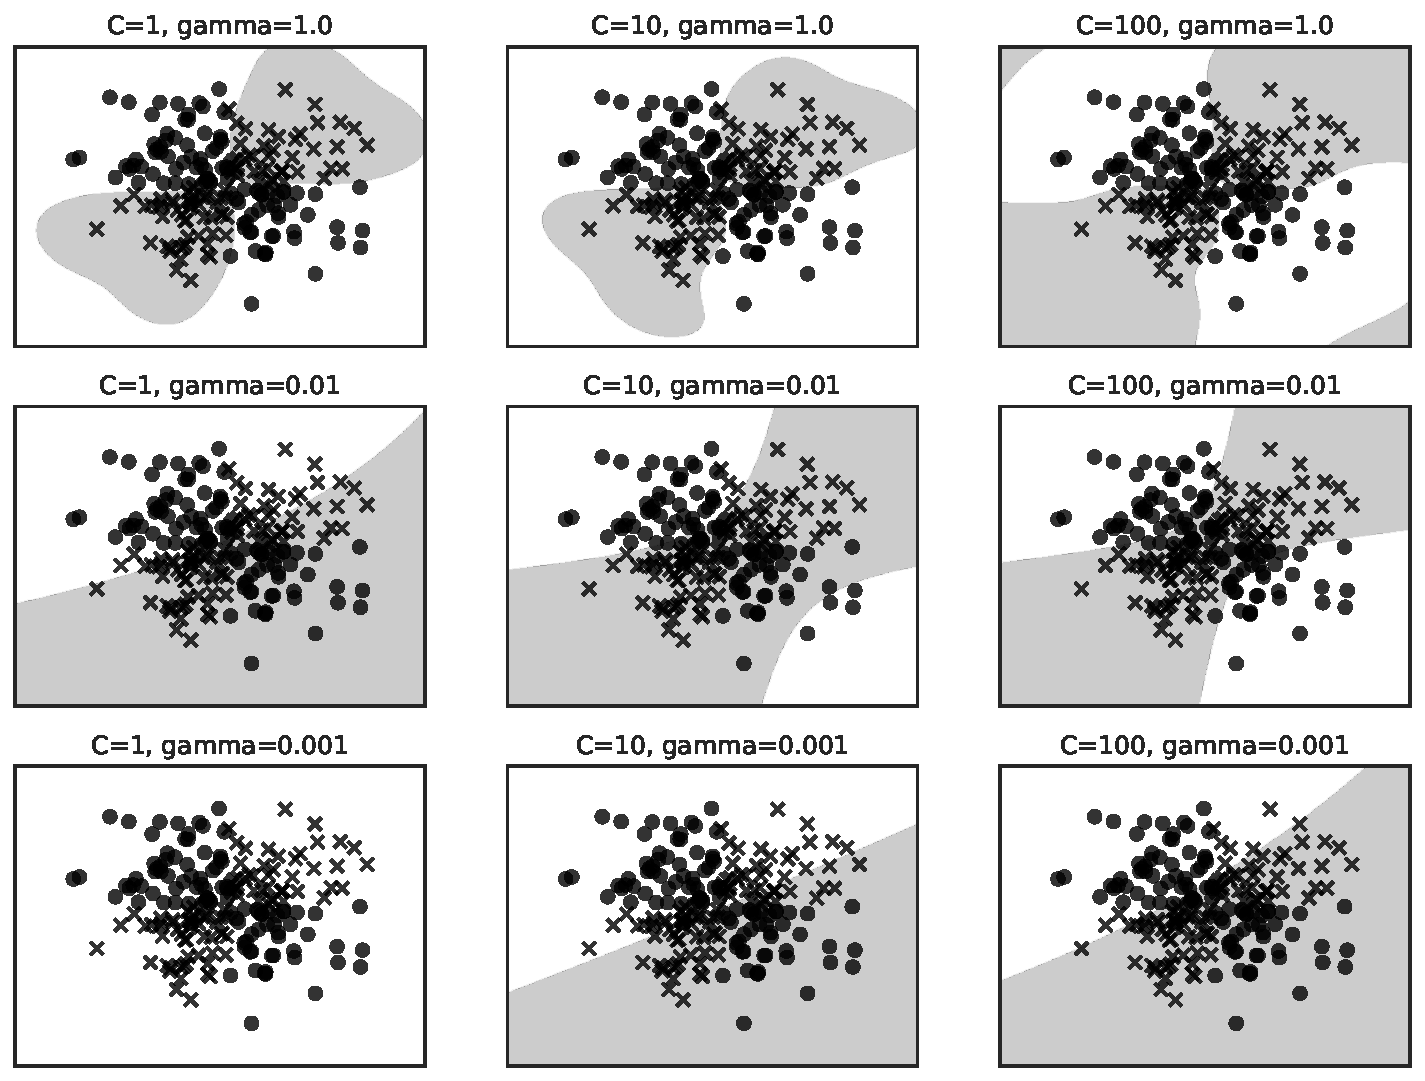
\includegraphics[width=0.85\textwidth]{appendix/svm_hyperparams}
    \caption{Effect of $C$ and $\gamma$ to the decision boundary}
  \label{demo:svm_hyperparams}
\end{figure}

\section{Distributed SVM Implementation}

\par In our work, SVM serves as the base classifier for the Binary-Relevance
(BR) algorithm. Recall that in BR, we take any ``off-the-shelf'' classifier and
train it $q$ times, where $q$ is the number of labels in the dataset. Most SVM
implementations have a time-complexity between $\mathcal{O}(N^2)$ and
$\mathcal{O}(N^3)$ (\cite{bottou2006support}).\footnote{We are using the
    \texttt{scikit-multilearn} library for BR and the \texttt{scikit-learn}
    library for SVM. Their SVM implementation is based on the \texttt{LIBSVM}
    solver by \cite{chang2011libsvm}.} 
With an overhead complexity brought by BR, our whole classifier algorithm can
take a long time to run.  Thus, we conducted a simple, distributed way of
training multiple SVM classifiers.

\par The main idea is to partition a dataset $\mathcal{D}$ into $K$ parts,
where $K \ll N$. We distribute each part into different jobs, i.e. each core of
the processor, and train it several times. Thus, given $q$ labels and $K$
partitions, we will have $K\cdot q$ smaller batches distributed on each core.
In practice, we limit the number of running cores to $10$ during
training.\footnote{The laboratory server's CPU has $40$ cores in total. This
can be confirmed by running \texttt{nproc --all} in the command line.} The
whole distributed process was implemented with the help of
\cite{varoquaux2010pipelines}'s \texttt{Pipelines} module (with
\texttt{multiprocessing} backend). Figure \ref{demo:distributed_svm} outlines
this process. When the \texttt{top} command is executed, we can see multiple
processes running inside the machine. A screenshot of this task is shown in
Figure \ref{demo:screenshot}.

\begin{figure}[t]
  \centering
    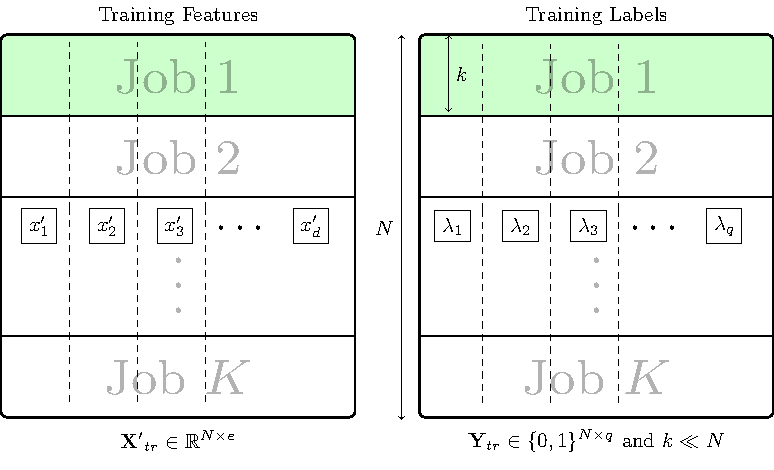
\includegraphics[width=0.70\textwidth]{appendix/distributed_svm}
    \caption[Distributed SVM training scheme]{Distributed SVM training
        scheme.\\ We partition the dataset into $K$ jobs, where $K\ll N$, and
    distribute it to different cores in our processor.}
  \label{demo:distributed_svm}
\end{figure}

\begin{figure}[!h]
  \centering
    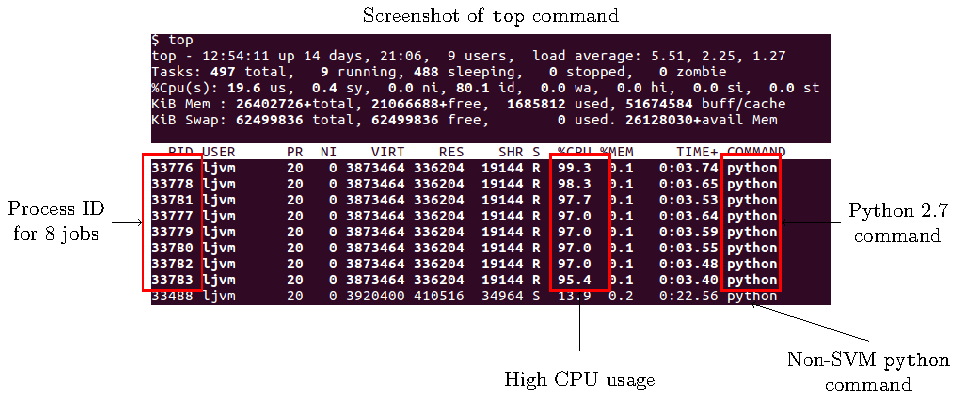
\includegraphics[width=0.95\textwidth]{appendix/parallel_compute}
    \caption[Screenshot of SVM jobs running in multiple cores]{Screenshot of
    SVM jobs running in multiple cores, $K=8$}
  \label{demo:screenshot}
\end{figure}

\par Lastly, we profiled this distributed approach by generating a toy multilabel
dataset and running it for different number of cores. For each step, we
measured the training time given different number of (1) samples, (2) features,
and (3) labels. Only the training time is measured because once the model is
fitted, inference is fast. The profiling results can be seen in Figure
\ref{demo:svm_profile}.

\begin{figure}[!t]
  \centering
    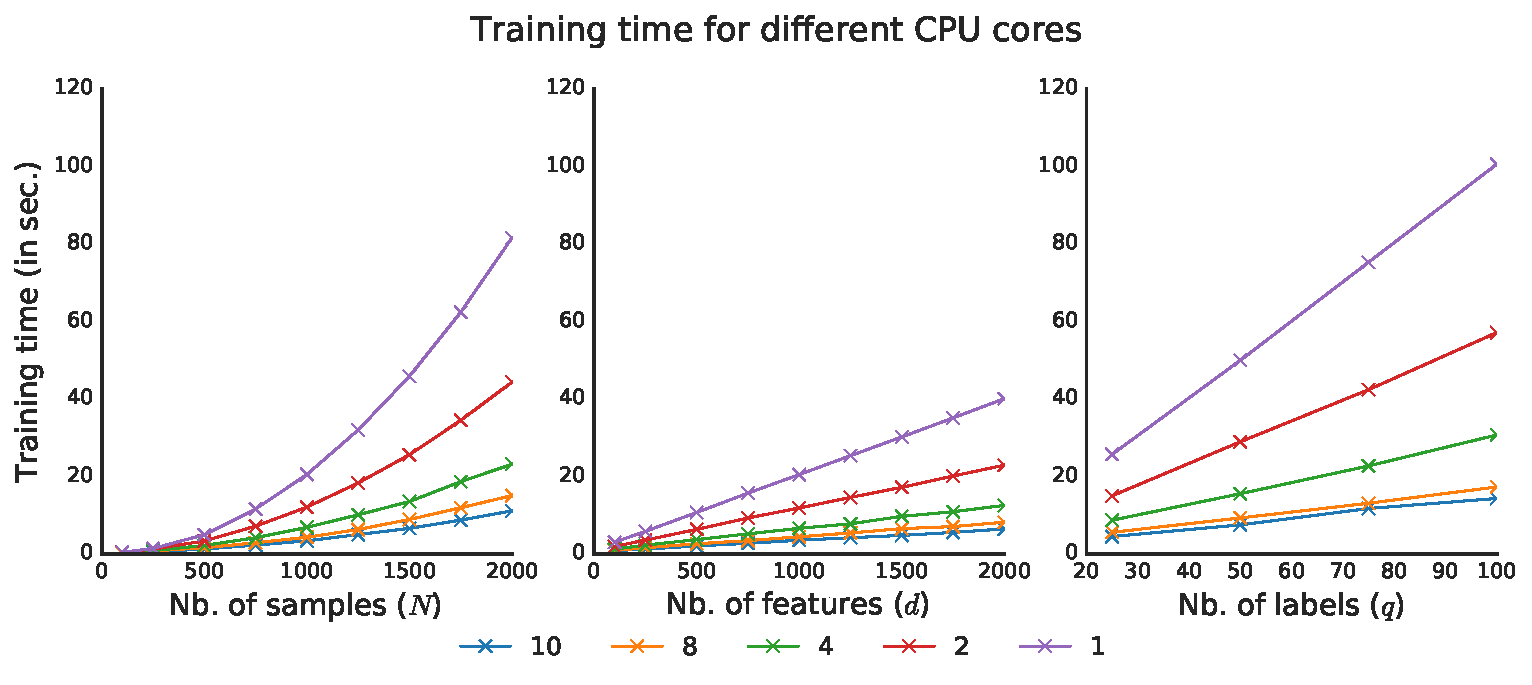
\includegraphics[width=0.95\textwidth]{appendix/svm_profile}
    \caption{Profiling results for SVM using different cores}
  \label{demo:svm_profile}
\end{figure}

\par It is evident that using the distributed approach reduces training time by
a large margin. The traditional approach ($K=1$) does not scale with large
datasets; it is more beneficial to use two or more cores for training. In
addition, we can also see the effect of different dataset sizes to the training
time. The curves in the leftmost plot shows an exponential relationship,
empirically validating the $\mathcal{O}(n^2)$ to $\mathcal{O}(n^3)$
time-complexity. On the other hand, the number of features ($d$) and labels
($q$) both exhibit a linear relationship with respect to the training time.
Either way, the curves above show that the distributed approach we have
implemented serves us in the long run. 
